\documentclass[12pt]{article}

\usepackage{amsmath,amsthm,amsfonts,amssymb,amsxtra}
\usepackage{pgf,tikz}
\usetikzlibrary{arrows}
\renewcommand{\theenumi}{(\alph{enumi})} 
\renewcommand{\labelenumi}{\theenumi}

\pagestyle{empty}
\setlength{\textwidth}{7in}
\setlength{\oddsidemargin}{-0.5in}
\setlength{\topmargin}{-1.0in}
\setlength{\textheight}{9.5in}

\newtheorem{problem}{Problem}

\begin{document}

\noindent{\large\bf MATH 141}\hfill{\large\bf Exam\#1.}\hfill{\large\bf
  Spring 2014}\hfill{\large\bf Page 1/6}\hrule

\bigskip
\begin{center}
  \begin{tabular}{|ll|}
    \hline & \cr
    {\bf Name: } & \makebox[12cm]{\hrulefill}\cr & \cr
    {\bf 4-digit code:} & \makebox[12cm]{\hrulefill}\cr & \cr
    \hline
  \end{tabular}
\end{center}
\begin{itemize}
\item Write your name and the last 4 digits of your SSN in the space provided above.
\item The test has six (6) pages, including this one.
\item Enter your answer in the box(es) provided.
\item You must show sufficient work to justify all answers unless
  otherwise stated in the problem.  Correct answers with inconsistent
  work may not be given credit.
\item Credit for each problem is given in parentheses at the right of
  the problem number.
\item No books, notes or calculators may be used on this test.
\end{itemize}
\hrule

\begin{center}
  \begin{tabular}{|c|c|c|}
    \hline
    &&\cr
    {\large\bf Page} & {\large\bf Max.~points} & {\large\bf Your points} \cr
    &&\cr
    \hline
    &&\cr
    {\Large 2} & \Large 20 & \cr
    &&\cr
    \hline
    &&\cr
    {\Large 3} & \Large 20 & \cr
    &&\cr
    \hline
    &&\cr
    {\Large 4} & \Large 20 & \cr
    &&\cr
    \hline
    &&\cr
    {\Large 5} & \Large 30 & \cr
    &&\cr
    \hline
    &&\cr
    {\Large 6} & \Large 10 & \cr
    &&\cr
    \hline\hline
    &&\cr
    {\large\bf Total} & \Large 100 & \cr
    &&\cr
    \hline
  \end{tabular}
\end{center}
\newpage

%%%%%%%%%%%%%%%%%%%%%%%%%%%%%%%%%%%%% Page 1
\noindent{\large\bf MATH 141}\hfill{\large\bf Exam\#1.}\hfill{\large\bf
  Spring 2014}\hfill{\large\bf Page 2/6}\hrule

\bigskip
{\problem[5 pts] \em Find $f(3)$ and $f(\pi)$ for}
$f(x) = 
\begin{cases}
 \sqrt{x+1} & \text{if } x\geq 1,\\
3 & \text{if } x<1.
\end{cases}$
\vspace{1cm}
\begin{flushright}
  \begin{tikzpicture}
    \draw (-1cm,0.5cm) node {$f(\pi) =$};
    \draw (0cm,0cm) rectangle (5cm,1.2cm);
    \draw (-1cm,2cm) node {$f(3) =$};
    \draw (0cm,1.4cm) rectangle (5cm,2.6cm);
  \end{tikzpicture}
\end{flushright}
\hrule
{\problem[10 pts] \em Find the domain and range of $f(x) = 2 + \sqrt{x-1}$.}
\vspace{4cm}
\begin{flushright}
  \begin{tikzpicture}
    \draw (-1cm,0.5cm) node {domain $=$};
    \draw (0cm,0cm) rectangle (5cm,1.2cm);
    \draw (-1cm,2cm) node {range $=$};
    \draw (0cm,1.4cm) rectangle (5cm,2.6cm);
  \end{tikzpicture}
\end{flushright}
\hrule
{\problem[5 pts] \em Sketch the graph of the function}
\begin{equation*}
f(x) = \begin{cases}  3- \tfrac{1}{2}x &\text{if } x\leq 2 \\ 2x-5 &\text{if } x>2 \end{cases}
\end{equation*}
\begin{center}
\begin{tikzpicture}
\draw[step=0.5cm, white!80!black, ultra thin] (-3.75cm,-3.75cm) grid (3.75cm,3.75cm);
\draw[black, ultra thick,<->] (0cm,-3.75cm) -- (0cm,3.75cm);
\draw[black, ultra thick,<->] (-3.75cm,0cm) -- (3.75cm,0cm);
\foreach \x in {-3,-2,-1,1,2,3}
	{
	\draw[ultra thick] (\x,-0.25cm) -- (\x, 0.25cm);
	\draw (\x, -0.5cm) node {$\x$};
	\draw[ultra thick] (-0.25cm, \x) -- (0.25cm, \x);
	\draw (-0.5cm,\x) node {$\x$};
	}
\end{tikzpicture}
\end{center}
\newpage

%%%%%%%%%%%%%%%%%%%%%%%%%%%%%%%%%%%%% Page 2
\noindent{\large\bf MATH 141}\hfill{\large\bf Exam\#1.}\hfill{\large\bf
  Spring 2014}\hfill{\large\bf Page 3/6}\hrule

\bigskip
{\problem[15 pts] \em Let $f(x) = x^2 + 3$ and $g(x) = \sqrt{x}$. Find
  $g \circ f$, $f \circ g$, and compute the domain of the latter.}
\vspace{9cm}
\begin{flushright}
  \begin{tikzpicture}
    \draw (-1.3cm,3.5cm) node {$ \big(g \circ f\big)(x) =$};
    \draw (0cm,2.8cm) rectangle (5cm,4cm);
    \draw (-1.3cm,2cm) node {$ \big(f \circ g\big)(x) =$};
    \draw (0cm,1.4cm) rectangle (5cm,2.6cm);
    \draw (-2.25cm,0.5cm) node {domain of $\big(f \circ g\big)(x) =$};
    \draw (0cm,0cm) rectangle (5cm,1.2cm);
  \end{tikzpicture}
\end{flushright}
\hrule
{\problem[5pts] \em Find the domain of the function $f(x) = \displaystyle{\frac{1}{1-e^x}}$.}
\vspace{5cm}
\begin{flushright}
\begin{tikzpicture}
    \draw (-1cm,0.5cm) node {domain $=$};
    \draw (0cm,0cm) rectangle (5cm,1.2cm);
\end{tikzpicture}
\end{flushright}
\newpage

%%%%%%%%%%%%%%%%%%%%%%%%%%%%%%%%%%%%% Page 3
\noindent{\large\bf MATH 141}\hfill{\large\bf Exam\#1.}\hfill{\large\bf
  Spring 2014}\hfill{\large\bf Page 4/6}\hrule

\bigskip
{\problem[5 pts] \em Solve for $x$:} \begin{equation*}\log (3x) - 3 \log (x^{-1/3}) =
  \log 27.\end{equation*}
\vspace{2cm}
\begin{flushright}
  \begin{tikzpicture}
    \draw (-0.75cm,0.5cm) node {$x =$};
    \draw (0cm,0cm) rectangle (5cm,1.2cm);
  \end{tikzpicture}
\end{flushright}
\hrule
{\problem[5 pts] \em Solve for $x$:} 
\begin{equation*}e^{5-3x} = 10.\end{equation*}
\vspace{2cm}
\begin{flushright}
  \begin{tikzpicture}
    \draw (-0.75cm,0.5cm) node {$x =$};
    \draw (0cm,0cm) rectangle (5cm,1.2cm);
  \end{tikzpicture}
\end{flushright}
\hrule
{\problem[10 pts] \em For the function $f$ with graph given below, state the value of each quantity, if it exists:}
\begin{center} 
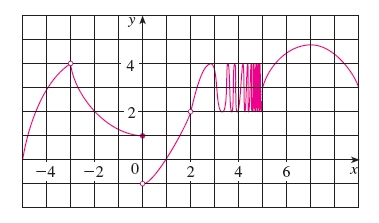
\includegraphics[width=0.5\linewidth]{gftest1}
\end{center}
\begin{eqnarray*}
\lim_{x\to -3^-} f(x)= \fbox{\hspace{0.5in}\strut}. & \lim_{x\to 0^+} f(x)= \fbox{\hspace{0.5in}\strut}. \\
\lim_{x\to -3^+} f(x)= \fbox{\hspace{0.5in}\strut}. & \lim_{x\to 0^-} f(x)=\fbox{\hspace{0.5in}\strut}. \\
\lim_{x\to -3} f(x)  = \fbox{\hspace{0.5in}\strut}.& \lim_{x \to 0} f(x)= \fbox{\hspace{0.5in}\strut}.
\end{eqnarray*}

\newpage

%%%%%%%%%%%%%%%%%%%%%%%%%%%%%%%%%%%%% Page 4
\noindent{\large\bf MATH 141}\hfill{\large\bf Exam\#1.}\hfill{\large\bf
  Spring 2014}\hfill{\large\bf Page 5/6}\hrule

\bigskip
{\problem[30 pts] \em Compute the following limits:}
\vspace{1cm}

\noindent
\begin{tikzpicture}
\draw (4cm,14cm) node{
(a) $\displaystyle{\lim_{x \to 1} \frac{x^2-2x-8}{x^2-4}} = \mbox{}$ };
\draw (6cm,13.4cm) rectangle (11cm,14.6cm);
\draw (4cm, 9cm) node{
(b) $\displaystyle{\lim_{x \to 2} \frac{x^2-2x-8}{x^2-4}} =
\mbox{}$}; 
\draw (6.1cm, 8.4cm) rectangle (11.1cm, 9.6cm); 
\draw (4cm, 2cm) node{
(c) $\displaystyle{\lim_{x \to 0} \frac{\sqrt{x+4}-2}{2x}} = \mbox{}$}; 
\draw (6cm, 1.4cm) rectangle (11cm, 2.6cm);
\end{tikzpicture}
\newpage


%%%%%%%%%%%%%%%%%%%%%%%%%%%%%%%%%%%%% Page 5
\noindent{\large\bf MATH 141}\hfill{\large\bf Exam\#1.}\hfill{\large\bf
  Spring 2014}\hfill{\large\bf Page 6/6}\hrule

\bigskip
{\problem[10 pts] \em Find the value of the constant $k$ for which the following function is continuous everywhere:}
\begin{equation*}
f(x) = \begin{cases}
2k^2x^3 &\text{if }x<2, \\
x+32k-18 &\text{if }x \geq 2.
\end{cases}
\end{equation*}
\vspace{16cm}
\begin{flushright}
  \begin{tikzpicture}
    \draw (-0.5cm,0.5cm) node {$k =$};
    \draw (0cm,0cm) rectangle (5cm,1.2cm);
  \end{tikzpicture}
\end{flushright}

\end{document}
